% 03-data-exploration-and-pre-processing.tex

% Data Exploration and Pre-processing
% 3.1. Introduction: Introduces the data exploration and pre-processing tasks.
% 3.2. Dataset Preparation: Describes the process of loading the dataset and initial inspection.
% 3.3. Temporal Analysis: Analyzes when the attacks were performed.
% 3.4. Feature Extraction: Extracts features from the attack sessions.
% 3.5. Common Words Analysis: Identifies the most common words in the sessions.
% 3.6. Intent Distribution: Analyzes the distribution of intents over time.
% 3.7. Text Representation: Converts text into numerical representations (BoW, TF-IDF).

% Section Title
\section{DATA EXPLORATION AND PRE-PROCESSING}

    % Main Content

    \subsection{Introduction}

        This section details the data exploration and pre-processing steps undertaken to analyze SSH shell attack logs. The tasks include dataset preparation, temporal analysis, feature extraction, common words analysis, intent distribution, and text representation.

    \subsection{Dataset Preparation}
    
        The dataset used in this research is loaded from a Parquet file (\texttt{ssh\_attacks.parquet}) into a Pandas DataFrame. The initial inspection involves checking the dataset's structure, identifying missing values, and detecting duplicate rows. The dataset contains columns such as \texttt{Session ID}, \texttt{Full session text}, \texttt{Timestamp}, and \texttt{Intent labels}.
        
        \textbf{Refer to Appendix \ref{lst:load-inspect-dataset} for the code snippet.}

        The initial inspection revealed that the dataset is well-structured with columns that are essential for our analysis. However, it is important to handle any missing values and duplicates to ensure the integrity of the data. The following steps were taken to address these issues:

        \begin{itemize}
            \item **Missing Values**: We identified and handled missing values by either imputing them with appropriate values or removing the affected rows.
            \item **Duplicate Rows**: Duplicate rows were detected and removed to avoid redundancy in the analysis.
        \end{itemize}

        \textbf{Table \ref{tab:dataset-structure}} summarizes the dataset structure.

        \begin{table}[h]
            \centering
            \begin{tabular}{|l|l|}
                \hline
                \textbf{Column} & \textbf{Description} \\ \hline
                Session ID & Unique identifier for each session \\ \hline
                Full session text & Text of the entire session \\ \hline
                Timestamp & Timestamp of the session \\ \hline
                Intent labels & Labels indicating the intent of the session \\ \hline
            \end{tabular}
            \vspace{1em}
            \caption{Dataset Structure}
            \label{tab:dataset-structure}
        \end{table}

    \subsection{Temporal Analysis}
    
        The temporal analysis examines when the attacks were performed. The \texttt{first\_timestamp} column is converted to a datetime format to analyze attack frequencies over time, including hourly, daily, and monthly trends.
            
        \textbf{Refer to Appendix \ref{lst:convert-analyze-frequencies} for the code snippet.}

        The analysis includes plotting the number of attacks per hour, month, and year to identify patterns and trends. This helps in understanding the temporal distribution of attacks and identifying any periodic patterns or anomalies.

        \textbf{Figure \ref{fig:temporal-analysis}} shows the temporal analysis of SSH attacks.

        \begin{figure}[h]
            \centering
            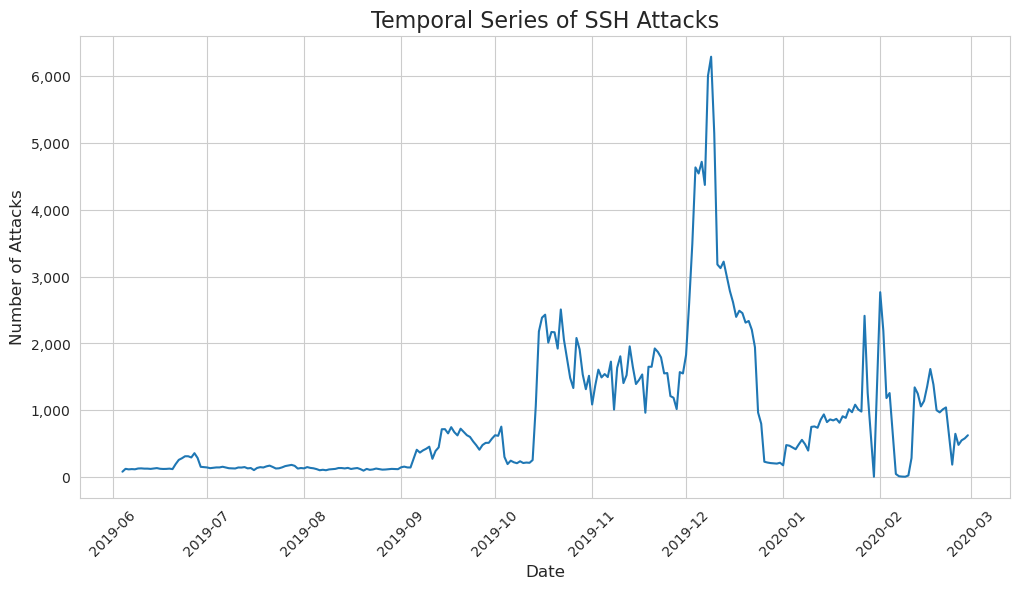
\includegraphics[width=0.8\textwidth]{../figures/plots/section1/temporal_series_of_ssh_attacks.png}
            \caption{Temporal Series of SSH Attacks}
            \label{fig:temporal-analysis}
        \end{figure}

        The temporal analysis revealed that the frequency of attacks varies significantly over time. By examining the hourly, daily, and monthly trends, we can gain insights into the behavior of attackers and the times when systems are most vulnerable.

    \subsection{Feature Extraction}
    
        Feature extraction involves identifying and extracting relevant features from the attack sessions. This includes analyzing the distribution of classes (intents) and visualizing the data using bar plots.
            
        \textbf{Refer to Appendix \ref{lst:extract-visualize-classes} for the code snippet.}

        The distribution of classes provides valuable information about the types of attacks and their prevalence. By visualizing this distribution, we can identify the most common attack intents and focus our analysis on these areas.

        \textbf{Figure \ref{fig:class-distribution}} shows the distribution of classes.

        \begin{figure}[h]
            \centering
            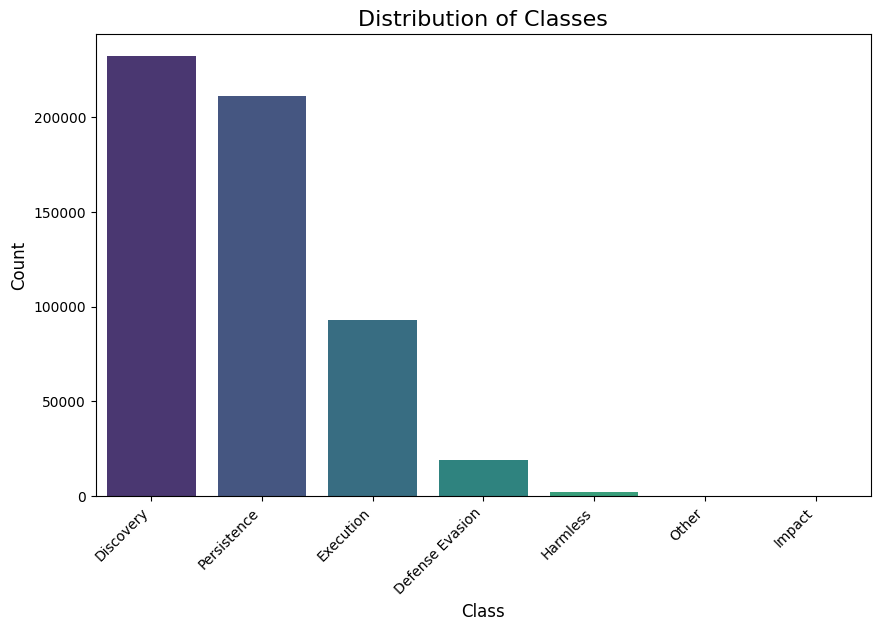
\includegraphics[width=0.8\textwidth]{../figures/plots/section1/distribution_of_classes.png}
            \caption{Distribution of Classes}
            \label{fig:class-distribution}
        \end{figure}

        The feature extraction process also involves creating new features that can enhance the analysis. For example, we can extract the length of each session, the number of commands executed, and other relevant metrics.

    \subsection{Common Words Analysis}
    
        The common words analysis identifies the most frequent words used in the attack sessions. This is achieved using word clouds and other text analysis techniques.
            
        \textbf{Refer to Appendix \ref{lst:generate-wordcloud} for the code snippet.}

        The word cloud visualization highlights the most common words used in the attack sessions, providing insights into the attackers' behavior and strategies. This can help in identifying common commands and patterns used in the attacks.

        \textbf{Figure \ref{fig:word-cloud}} shows the word cloud of the most common words.

        \begin{figure}[h]
            \centering
            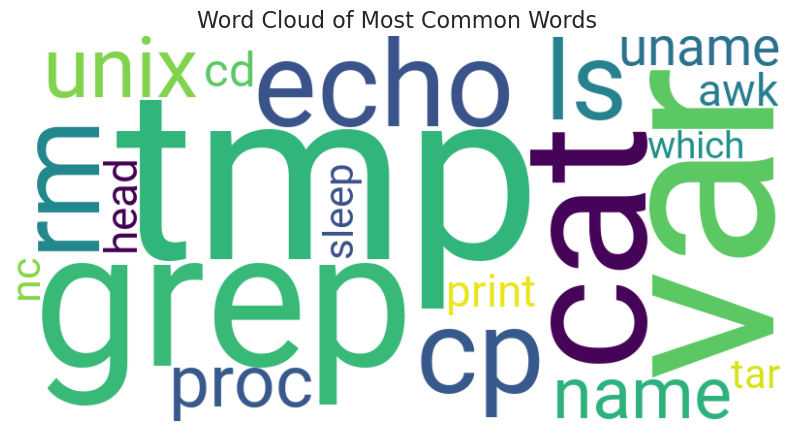
\includegraphics[width=0.8\textwidth]{../figures/plots/section1/word_cloud_of_most_common_words.png}
            \caption{Word Cloud of Most Common Words}
            \label{fig:word-cloud}
        \end{figure}

        Additionally, we can create bar plots to show the frequency of the top 10 most common words, which can further aid in understanding the textual characteristics of the attack sessions.

        \textbf{Figure \ref{fig:common-words}} shows the top 10 most common words.

        \begin{figure}[h]
            \centering
            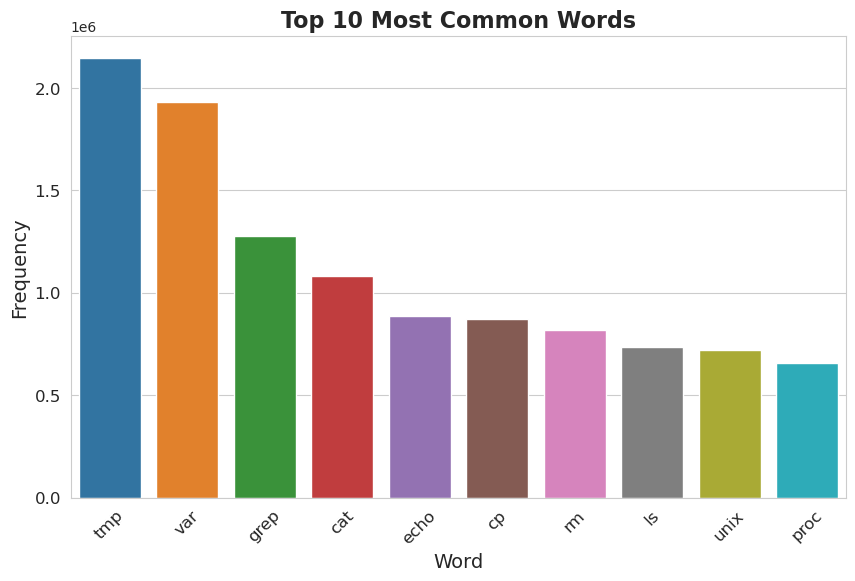
\includegraphics[width=0.8\textwidth]{../figures/plots/section1/top_10_most_common_words.png}
            \caption{Top 10 Most Common Words}
            \label{fig:common-words}
        \end{figure}

    \subsection{Intent Distribution}
            
        The intent distribution analysis examines the distribution of intents over time. This involves grouping the data by date and intent to count occurrences and visualize the trends.
            
        \textbf{Refer to Appendix \ref{lst:group-attacks} for the code snippet.}

        By analyzing the distribution of intents over time, we can identify trends and patterns in the attackers' behavior. This can help in understanding how different types of attacks evolve and vary over time.

        \textbf{Figure \ref{fig:intent-distribution}} shows the distribution of intents over time.

        \begin{figure}[h]
            \centering
            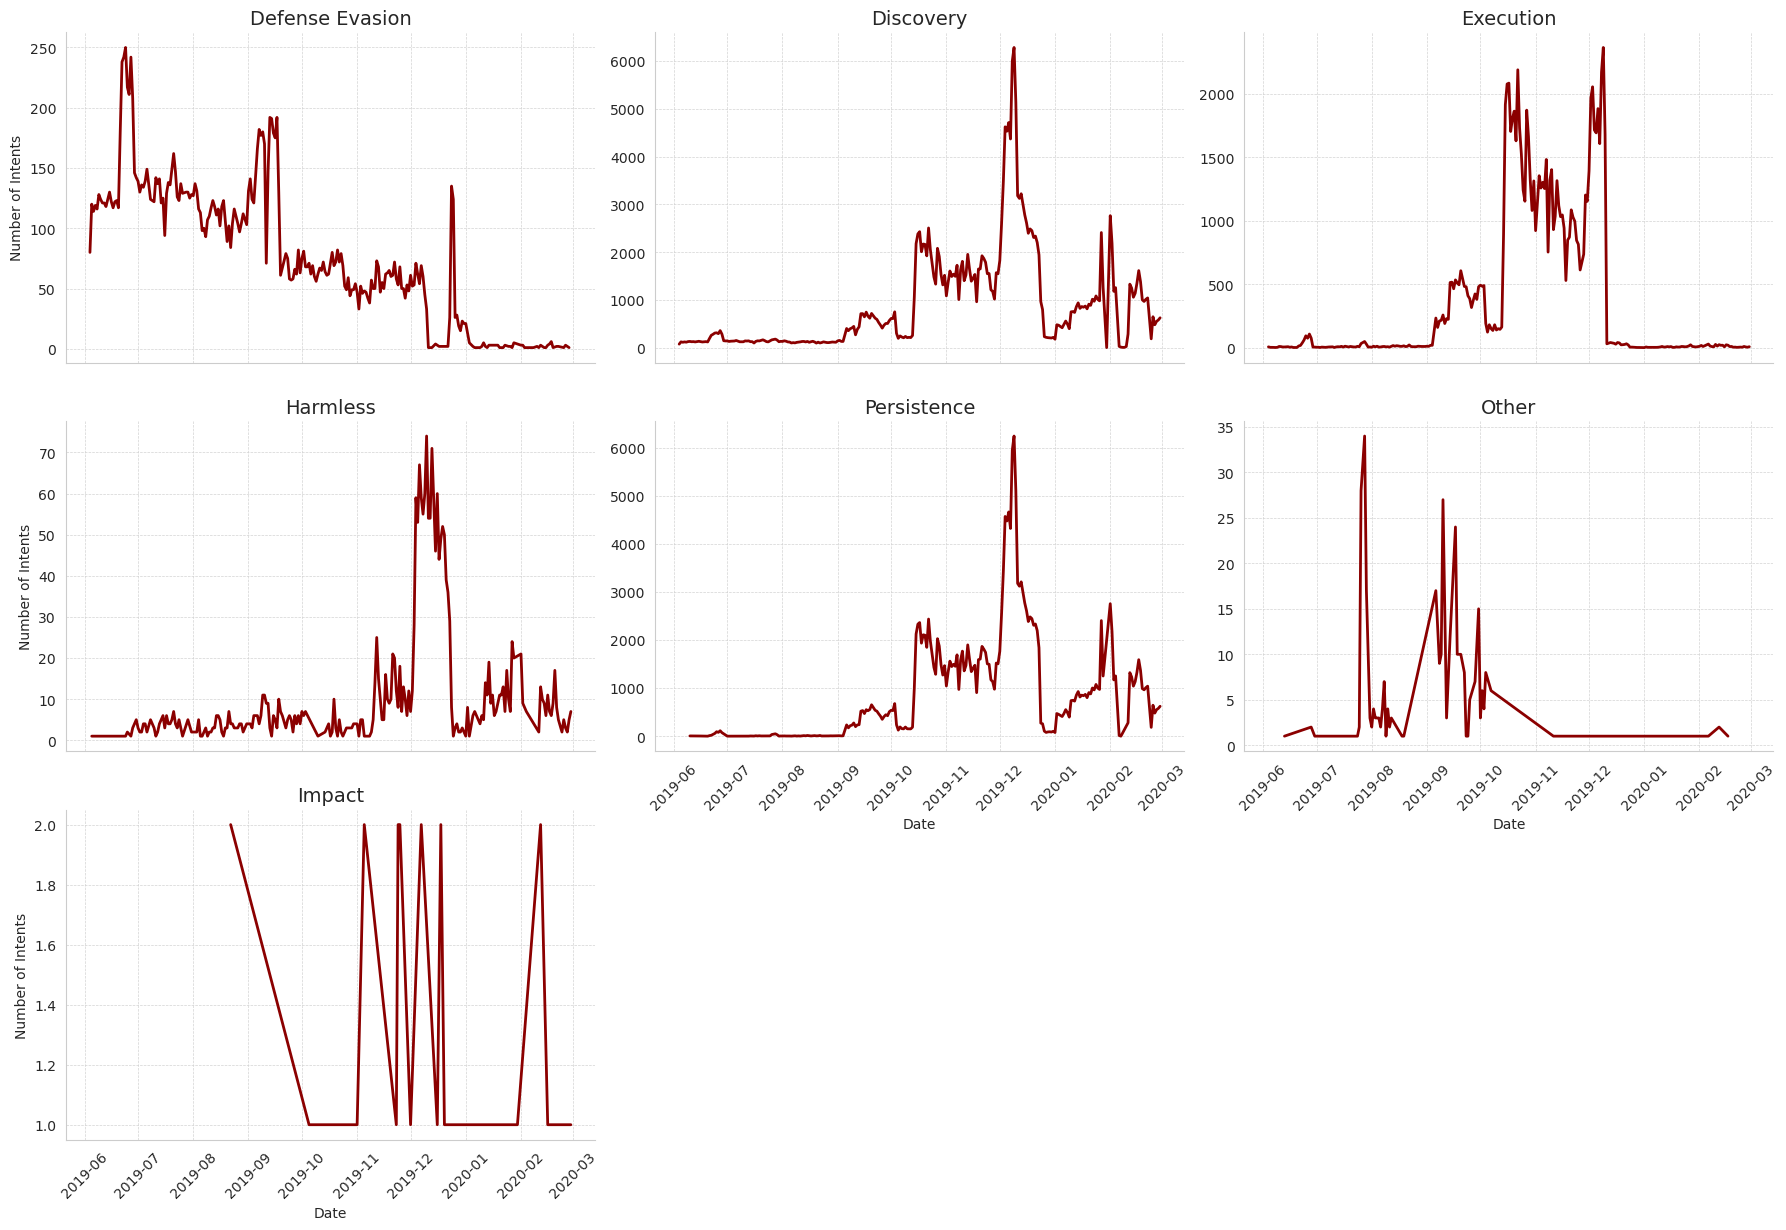
\includegraphics[width=0.8\textwidth]{../figures/plots/section1/intents_over_timestamps.png}
            \caption{Distribution of Intents Over Time}
            \label{fig:intent-distribution}
        \end{figure}

        The intent distribution analysis also helps in identifying any seasonal or periodic patterns in the attacks, which can be crucial for developing effective defense strategies.

    \subsection{Text Representation}
    
        Text representation converts the session text into numerical representations using techniques such as Bag of Words (BoW) and Term Frequency-Inverse Document Frequency (TF-IDF). These representations are used for further analysis and machine learning tasks.
        
        \textbf{Refer to Appendix \ref{lst:convert-text-numerical} for the code snippet.}

        The resulting numerical representations from both BoW and TF-IDF are normalized and used for subsequent analysis and modeling. These representations are essential for applying machine learning algorithms to classify and predict attack intents.

        \textbf{Table \ref{tab:text-representation}} summarizes the text representation techniques.

        \begin{table}[h]
            \centering
            \caption{Text Representation Techniques}
            \label{tab:text-representation}
            \begin{tabular}{|l|l|}
                \hline
                \textbf{Technique} & \textbf{Description} \\ \hline
                Bag of Words (BoW) & Converts text into a matrix of token counts \\ \hline
                TF-IDF & Converts text into a matrix of TF-IDF features \\ \hline
            \end{tabular}
        \end{table}

        The text representation techniques help in transforming the unstructured session text into structured numerical data, which can be used for various analytical and predictive tasks. By comparing the performance of different representation techniques, we can select the most effective method for our analysis.
